%%%%%%%%%%%%%%%%%%%%%%% file template.tex %%%%%%%%%%%%%%%%%%%%%%%%%
%
% This is a general template file for the LaTeX package SVJour3
% for Springer journals.          Springer Heidelberg 2010/09/16
%
% Copy it to a new file with a new name and use it as the basis
% for your article. Delete % signs as needed.
%
% This template includes a few options for different layouts and
% content for various journals. Please consult a previous issue of
% your journal as needed.
%
%%%%%%%%%%%%%%%%%%%%%%%%%%%%%%%%%%%%%%%%%%%%%%%%%%%%%%%%%%%%%%%%%%%
%
% First comes an example EPS file -- just ignore it and
% proceed on the \documentclass line
% your LaTeX will extract the file if required
%\begin{filecontents*}{example.eps}
%%!PS-Adobe-3.0 EPSF-3.0
%%%BoundingBox: 19 19 221 221
%%%CreationDate: Mon Sep 29 1997
%%%Creator: programmed by hand (JK)
%%%EndComments
%gsave
%newpath
%  20 20 moveto
%  20 220 lineto
%  220 220 lineto
%  220 20 lineto
%closepath
%2 setlinewidth
%gsave
%  .4 setgray fill
%grestore
%stroke
%grestore
%\end{filecontents*}
%
\RequirePackage{fix-cm}
%
%\documentclass{svjour3}                     % onecolumn (standard format)
%\documentclass[smallcondensed]{svjour3}     % onecolumn (ditto)
%\documentclass[smallextended]{svjour3}       % onecolumn (second format)
\documentclass[twocolumn]{svjour3}          % twocolumn
%
\smartqed  % flush right qed marks, e.g. at end of proof
%
\clubpenalty=10000
\widowpenalty = 10000
\usepackage{CJK}
\usepackage{amsmath}
\usepackage{array}
\usepackage{setspace}
\usepackage[lined,linesnumbered,ruled]{algorithm2e}
\newcommand\mycommfont[1]{\footnotesize\ttfamily\textcolor{blue}{#1}}
\SetCommentSty{mycommfont}
\usepackage{algorithmic}
\usepackage{color}
\usepackage{enumitem}
\usepackage{url}
\usepackage[footnotesize]{subfigure}
\renewcommand{\arraystretch}{1.5}
%\usepackage[pagebackref=true,breaklinks=true,letterpaper=true,colorlinks,bookmarks=false]{hyperref}
\usepackage{hyperref}
\hypersetup{colorlinks=false,linkcolor=blue,urlcolor=blue,citecolor=red}
%\usepackage[labelfont=bf, textfont=bf]{caption}
\usepackage{tabularx}



\usepackage{relsize}
\usepackage{dsfont}
%\usepackage{hologo}[2012/04/26]
\usepackage[footnotesize]{subfigure}
\usepackage{mathtools}
\newcommand{\defeq}{\vcentcolon=}
\newcommand{\inv}{^{\raisebox{.2ex}{$\scriptscriptstyle-1$}}} 
\newcommand{\eg}{\textit{e.g.}}
\newcommand{\ie}{\textit{i.e.}}
\newcommand{\sgn}{\textrm{sgn}}
\newcommand{\etal}{~\textit{et al.}}
%
% \usepackage{mathptmx}      % use Times fonts if available on your TeX system
%
% insert here the call for the packages your document requires
%\usepackage{latexsym}
% etc.
%
% please place your own definitions here and don't use \def but
% \newcommand{}{}
%
% Insert the name of "your journal" with
% \journalname{myjournal}
%
\begin{document}

\title{Visual Knowledge Representation Learning
}
\subtitle{A Survey Towards Briding the Semantic Gap by Connecting Language and Vision}

\author{Hanwang Zhang         \and
        Zhiyuan Liu\and
        Tat-Seng Chua
}

\institute{Hanwang Zhang \at
              School of Computing, National University of Singapore \\
              \email{hanwangzhangr@gmail.com}           %  \\
           \and
           Zhiyuan Liu \at
           Department of Computer Science, Tsinghua University\\
           \email{liuzy@tsinghua.edu.cn}
           \and
           Tat-Seng Chua \at
           School of Computing, National University of Singapore \\
           \email{dcscts@nus.edu.sg}
}

\date{Received: date / Accepted: date}
% The correct dates will be entered by the editor


\maketitle

\begin{abstract}
Here, I simply describe some motivations of the title and the paper organization. You are more than welcomed to give comments.

First, I think all of us might agree on the main title; for the subtitle, I use the most classic term ``semantic gap'' in multimedia to highlight the fundamental impact of this survey. By using ``connecting language and vision'', which is the trending topic in both multimedia and computer vision, I would like to highlight that our survey is more focused on the recent progress on the marriage of NLP and CV.

Second, organizations are listed as section titles, followed by some informal descriptions of a section. Some seed references are also cited.

\keywords{Semantic Gap \and Knowledge Base \and Representation Learning \and Natural Language Processing \and Computer Vision}
% \PACS{PACS code1 \and PACS code2 \and more}
% \subclass{MSC code1 \and MSC code2 \and more}
\end{abstract}

\section{Introduction}\label{sec:1}
\begin{figure}
	\centering
	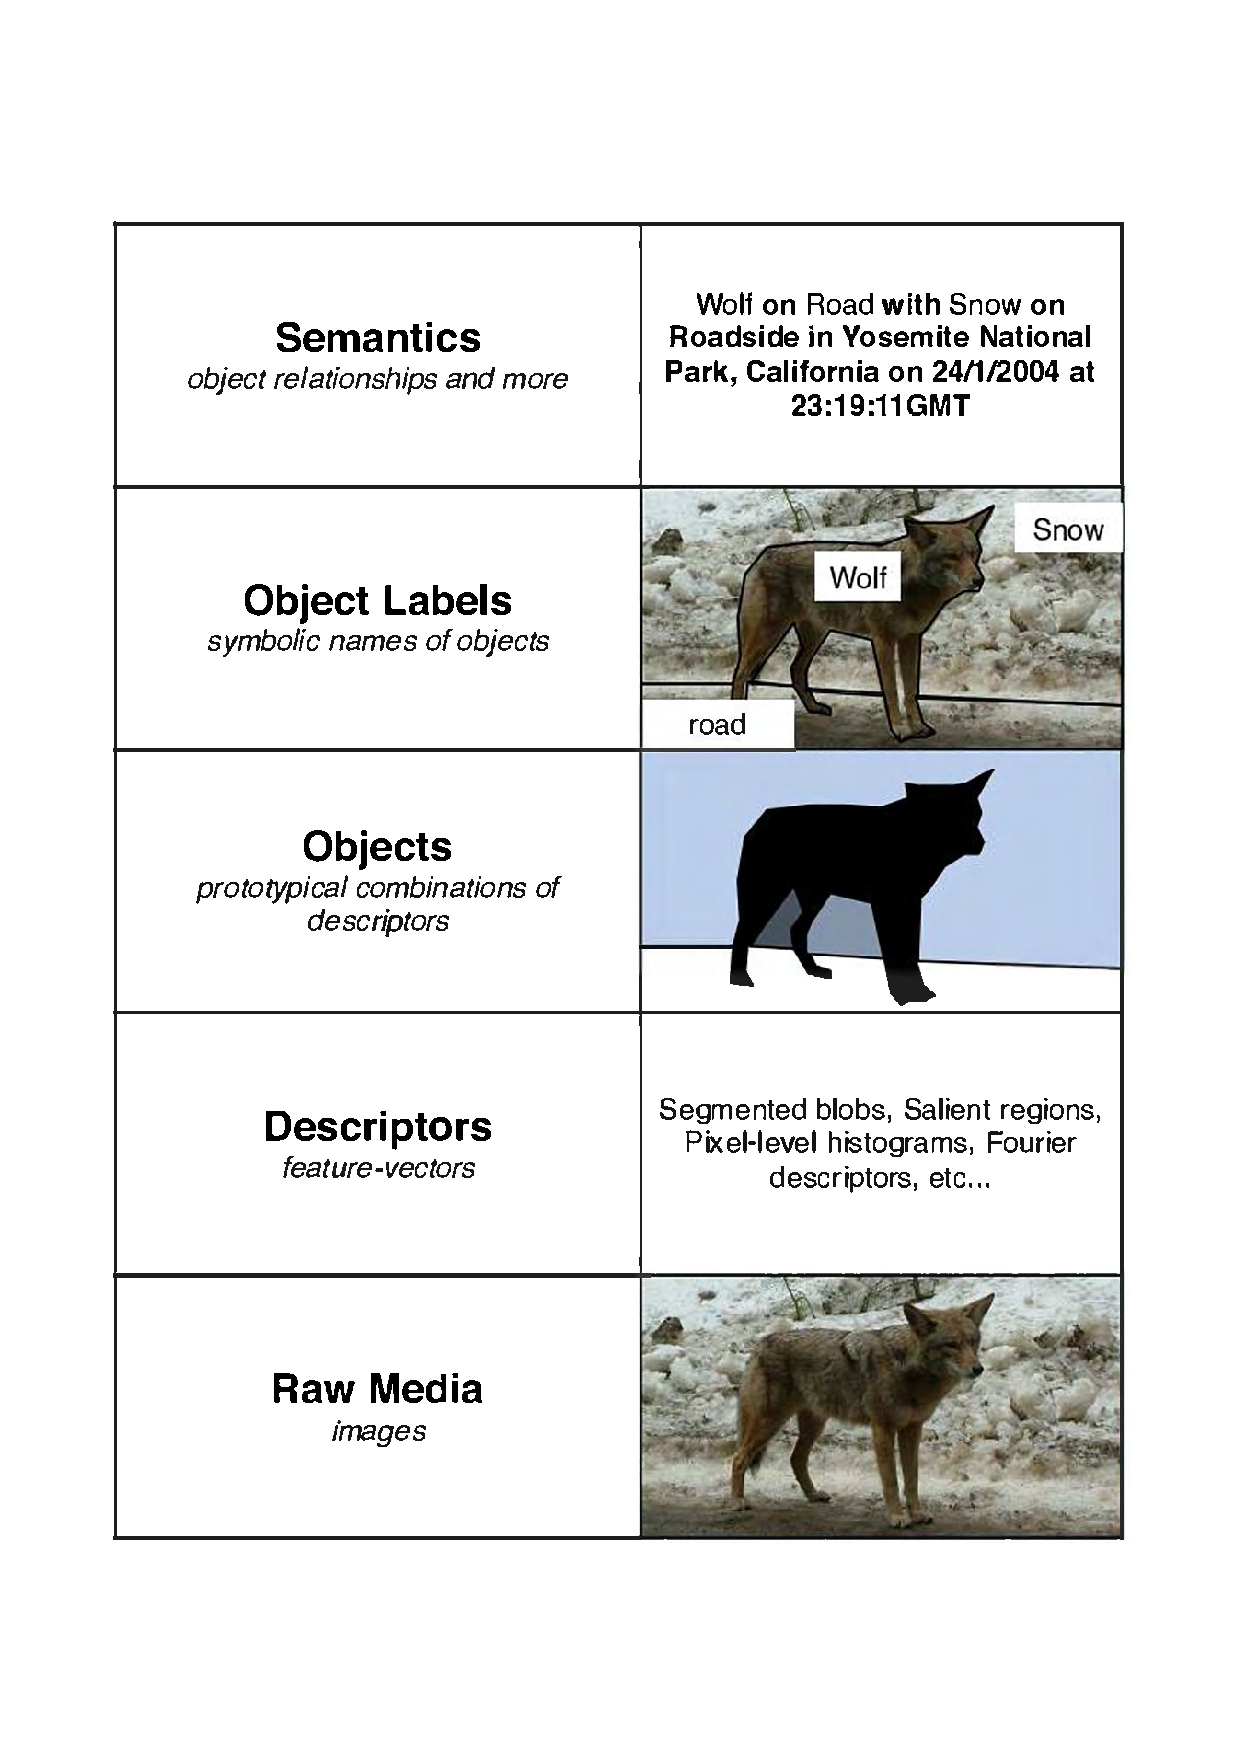
\includegraphics[width=1\linewidth]{figure/1.pdf}
	\caption{The Semantic Gap: Hierarchy of levels between the raw media and full semantics.}
	\label{fig:1}
\end{figure}
1. We recall the ever-lasting \emph{Semantic Gap} in multimedia community, since the very well-known Smeulders' survey paper~\cite{smeulders2000content}. Semantic gap states the challenge that the low-level visual features are usually unable to encode all the semantics needed for end tasks such as image retrieval and classification. 
2. Our community, the main goal of multimedia analytics is to bridge this gap, benefiting any forms of multimedia information retrieval. Techniques that tackle this, can be categorized into the following three areas:
\begin{itemize}[leftmargin=*]
	\item \textbf{Visual Features}. Visual features represent an image as vectors, which are the most effective and efficient way for visual representations. However, it is also vulnerable to variations in visual world, which result in large semantic gap. Fortunately, recent progress in deep learning has impressively robustify the features.
	\item \textbf{Semantic Concepts}. Visual features are not human interpretable and thus inevitably hinders the user-content interactions. To achieve this, building a set of semantic concepts is a promising way, which is widely used in TRECVID events. However, these semantics are unstructured and thus do not provide deep understanding of images. 
	\item \textbf{Semantic Descriptions}. A full semantic description for an image such as objects, relations among objects and even the background knowledge of them, is our ultimate goal.
\end{itemize}

Figure~\ref{fig:1} from~\cite{hare2006mind} illustrates where the semantic resides in content understanding. With the development of CV, we can do well from the first level to the fourth level, however, the fifth level is still an open issue, which we claim that it should be resolved with a Visual Knowledge Base (VKB). And we believe the timing is ripe to do such research.

Talk about why we use a knowledge base for visual representation. Briefly introduce the recent progresses in NLP and CV that exploit knowledge base.

Paper organizations.

\section{Visual Semantics}\label{sec:2}
In this section, we briefly review our efforts made to bridge the semantic gaps in the past two decades. Generally, they are various of semantic classifiers trained for describing images.

The methods introduced in this section is generally based on classification paradigm. Compared to the rich reasoning that can go through a person's mind upon seeing an object, a typical object classifier is doing a ``shallow'' reasoning and hence results in limited semantic understanding. 

\subsection{Concepts}
High-level semantic concepts
\subsection{Attributes}
Intermediate-level concepts. These two sections can be found in my PhD thesis.
\subsection{Relations}
Such as actions, verbs, or other interactive semantics. These semantics are rarely investigated in CV and MM.

\section{Knowledge Base}\label{sec:3}
I think Zhiyuan can organize this.

\section{Visual Knowledge Base}\label{sec:4}
Inspired by the KB advances in NLP, the CV community has recently begun to explore Visual Knowledge Base (VKB).

Once again highlight the necessity of building VKB. For example, the incomplete VKB: ImageNet, has greatly pushed the development of CV in recent years.

\subsection{Existing Organizations}\label{sec:4_1}
Introduce some existing VKB organizations.
\subsubsection{Visual Data Population to Existing Knowledge Base}\label{sec:4_1_1}
Based on existing KB, such as WordNet, we populate images according to the base. Such as the well-known ImageNet, and the two outdated projects: LSCOM and Vispedia. In fact, any visual datasets with labels can be considered as VKB of this kind.
\subsubsection{Image as Entities}\label{sec:4_1_3}
The above KBs considered conventional concepts as entities. In~\cite{zhu2015building}, they consider each single image as an entity. But I think it is not a principled way.
\subsubsection{Others}\label{sec:4_1_4}



\subsection{Constructions}\label{sec:4_2}
How to build a VKB. A good VKB should be \textbf{Large Scale} (this may require automatic techniques), \textbf{Well structured} and \textbf{Incremental} (easy for insertion and deletion). Zhiyuan may define in a more formal way of what a VKB should be like.
\subsubsection{Crowdsourcing}\label{sec:4_2_1}
Invite human labelers to annotate, such as ImageNet, and the recent Visual Genome~\cite{krishna2016visual}.

\subsubsection{Automatic Semantic Discovery}\label{sec:4_2_2}
Discovering semantic concepts and hierarchies from Web data. This is the Webly-Discovered knowledge base. Most of them are merely noisy but automatically discovered datasets, such as NEIL~\cite{chen2013neil,chen2015webly}, my MM14 paper~\cite{zhang2014start}, Microsoft ImageKB~\cite{wang2012towards}, LEVAN~\cite{divvala2014learning}. But few of them have rich relations among entities.

\subsubsection{Automatic Relation Verification}\label{sec:4_2_3}
Discovering relations from web data. Such as mining object affordances~\cite{zhu2014reasoning,chao2015mining} and relation verifications~\cite{vedantam2015learning,sadeghi2015viske}. 


\section{Visual Knowledge Representation Learning}\label{sec:5}
Why learning a representation is necessary? In other words, we want to know how to use VKB in a computational way: how to ground images? how to predict semantic facts given an image using VKB? Yet, unfortunately, there is no principled way in VKB. This might be a chance for us to develop.
\subsection{Knowledge Grounding and Inference}
Grounding entities in KB to visual regions (\eg, objects) of images~\cite{johnson2015image}. Almost all the above papers introduce somewhat ad-hoc methods. Formulations for inference. Given the visual information provided by the image (\ie, after grounding), can we get the semantic description of the image as complete as possible?
\subsection{Learning Models}
Formulations for training.
\subsubsection{Graphical Models}
\subsubsection{Distributional Representations}


\section{Discussions and Future Directions}\label{sec:6}
\subsection{Our proposals?}
I feel that we should establish a principled framework for (a) VKB's construction: existing KB+automatic visual population, \eg, mapping VisualGenome dataset~\cite{krishna2016visual} or ImageNet to Zhiyuan's KB; and (b) joint or partial learning the VKB, \eg, although partial entities and relations are annotated with images, how can we propagate the visual information to/ or exploit the rest KB to enhance the power of VKB? 

In fact, in~\cite{zhu2014reasoning}, it seems that it is a joint learning (every two entities have a weight to be learned) of visual evidence (\eg, image visual features or its induced binary classifiers as weight and human pose estimations) and predefined rules in KB (\eg, affordance edges, attribute assigning probabilities), using Markov Logic Network.

Interestingly, here is a recent scene graph parser that is compatible to the format of VisualGenome, called Standford Scene Graph Parser~\cite{schuster2015generating}

\subsection{Visual Feature Enrichment}
Use VKB to enrich existing visual features
\subsection{Visual QA}
\subsection{Retrieval with Complex Multimedia Query} A query with text and image.
\subsection{Semantic Video Description}
Video is a higher-order multimedia content, how to represent it in a KB.
\subsection{Incorporating Social Curation}
Social intelligence can curate noisy but abundant visual informations for KB. How can we take advantage of it?



\bibliographystyle{abbrv}
{\scriptsize{\bibliography{vkb}}}

\end{document}
% end of file template.tex

